% ------------------------------------------------------------------
\renewcommand{\thisweek}{MATH327 Week 4}
\renewcommand{\moddate}{Last modified 20 Feb.~2021}
\setcounter{section}{4}
\setcounter{subsection}{0}
\phantomsection
\addcontentsline{toc}{section}{Week 4: Ideal gases}
\section*{Week 4: Ideal gases}

\subsection{Volume, energy levels, and partition function}
This week we apply the canonical ensemble to investigate non-relativistic, classical, ideal gases.
Using statistical physics we will explore how the large-scale behaviours of such gases emerge from the properties of the particles that compose them.
The three adjectives above specify these properties in the case we consider this week: \\[-24 pt]
\begin{itemize}
  \item \textbf{Classical} systems are those for which we can ignore the effects of quantum mechanics.
        At a technical level, this means we assume we can simultaneously define both the position $(x, y, z)$ and the momentum $\vec p = (p_x, p_y, p_z)$ of each particle with arbitrary precision.
  \item \textbf{Non-relativistic} particles move with speeds small compared to the speed of light, which allows us to ignore small effects due to special relativity.
        The particles are therefore governed by the laws Isaac Newton published all the way back in 1687.
        In particular, the energy of each particle of mass $m$ is
        \begin{equation*}
          E_n = \frac{1}{2m} p_n^2,
        \end{equation*}
        where $p_n^2 = \vec p_n \cdot \vec p_n = (p_x)_n^2 + (p_y)_n^2 + (p_z)_n^2$ is the inner (or `dot') product of the momentum vector for the $n$th particle.
  \item \textbf{Ideal} gases are those whose constituent particles don't interact with each other.
        As a result, the total energy of the gas is simply the sum of the energies of the $N$ individual particles,
        \begin{equation}
          E = \frac{1}{2m} \sum_{i = n}^N p_n^2.
        \end{equation}
\end{itemize}

As usual for the canonical ensemble, we consider the gas to be in thermodynamic equilibrium, and in thermal contact with a large external thermal reservoir with which it can exchange energy but not particles.
To prevent particle exchange, we can specify that the gas is enclosed in a box with volume $V = L^3$.
The thermal reservoir fixes the temperature $T$ of the gas.

The starting point for our analysis is to compute the partition function
\begin{equation*}
  Z = \sum_i e^{-E_i / T}.
\end{equation*}
Here the sum is over all possible micro-states $\om_i$ of the $N$-particle system, which is problematic.
These micro-states depend on the momenta $\vec{p}_n$ for all $N$ particles, and it's intuitive to suppose that each component of $(p_x, p_y, p_z)_n$ is a continuously varying real number that can (in principle) be distinguished with arbitrary precision.
This implies an uncountably infinite set of distinct momenta and hence an uncountably infinite set of micro-states, making the summation above ill-defined.

To proceed, we need to \textit{regulate} the system so that there are a countable number of micro-states and we can define the partition function.
We do this by positing that the particles' momentum components can take only discrete (or `quantized') values that depend on the volume of the box.
Specifically, we declare that the possible momenta are
\begin{align}
  \label{eq:quant_mom}
  \vec p & = (p_x, p_y, p_z) = \hbar \frac{\pi}{L} (k_x, k_y, k_z) &
  k_{x, y, z} = 0, 1, 2, \cdots.
\end{align}
Each component of the non-negative-integer vector $\vec k = (k_x, k_y, k_z)$ is independent.
The constant factor $\hbar$ (``h-bar''), known as the (reduced) Planck constant (named after \href{https://en.wikipedia.org/wiki/Max_Planck}{Max Planck}), simply converts units from inverse-length ($\frac{1}{L}$) to momentum ($p$).
Very similar discrete momenta turn out to be realized in nature, thanks to quantum mechanics---if you have previously studied quantum physics, you may recognize the momenta for a \href{https://en.wikipedia.org/wiki/Particle_in_a_box}{particle in a box}, but for the purposes of this module we can just adopt this result as an ansatz.

What are the energies that correspond to these discretized momenta?
\begin{mdframed}
  \ \\[50 pt]
\end{mdframed}
You should find energies that fall into discrete \textit{energy levels}, somewhat similar to the spin system considered last week.

Even though there are still an infinite number of possible momenta and energy levels for each particle in the gas, these are now countable, making our partition function well-defined.
Let's start by considering the partition function $Z_1$ for a single particle in the box.
The micro-states for this single-particle system are completely specified by that particle's momentum $\vec p$,
\begin{equation*}
  Z_1 = \sum_i \exp\left[-\frac{E_i}{T}\right] = \sum_{\vec p} \exp\left[-\frac{p^2}{2mT}\right] = \sum_{k_{x, y, z} = 0}^{\infty}\exp\left[-\frac{\hbar^2 \pi^2}{2mTL^2}\left(k_x^2 + k_y^2 + k_z^2\right)\right].
\end{equation*}
Because $(k_x, k_y, k_z)$ are all independent, we can sum over each of them independently,
\begin{equation*}
  Z_1 = \sum_{k_x = 0}^{\infty} \exp\left[-\frac{\hbar^2 \pi^2}{2mTL^2} k_x^2\right] \sum_{k_y = 0}^{\infty} \exp\left[-\frac{\hbar^2 \pi^2}{2mTL^2} k_y^2\right] \sum_{k_z = 0}^{\infty} \exp\left[-\frac{\hbar^2 \pi^2}{2mTL^2} k_z^2\right].
\end{equation*}

For technical reasons,\footnote{If $m$ is too small, effects due to special relativity become non-negligible.  If $T$ is too small, effects due to quantum physics become non-negligible.  If $L$ is too small, we don't have a sufficiently large-scale  (\textit{macroscopic}) system to justify analysis via statistical ensembles in the first place.} the three properties listed above allow us to assume that Planck's constant $\hbar$ is extremely small compared to $L\sqrt{mT}$, so that
\begin{equation*}
  \frac{\hbar^2 \pi^2}{2mTL^2} \ll 1.
\end{equation*}
This means that the energy levels are spaced very close to each other, and the summations over discrete integer $k$ can be well approximated by integrals over continuous real $\khat$, so that
\begin{equation*}
  \sum_{k_x = 0}^{\infty} \exp\left[-\frac{\hbar^2 \pi^2 k_x^2}{2mTL^2}\right] \approx \int_0^{\infty} d\khat_x \exp\left[-\frac{\hbar^2 \pi^2 \khat_x^2}{2mTL^2}\right] = \frac{1}{2} \int_{-\infty}^{\infty} d\khat_x \exp\left[-\frac{\hbar^2 \pi^2 \khat_x^2}{2mTL^2}\right].
\end{equation*}
The final equality simply notes that the integrand is an even function of $\khat_x$ (depending only on $\khat_x^2$).

Since we're back to working with continuous real momenta, we may as well use \eq{eq:quant_mom} to return to the original $dp_x = \hbar \frac{\pi}{L} d\khat_x$,
\begin{equation*}
  \sum_{k_x = 0}^{\infty} \exp\left[-\frac{\hbar^2 \pi^2}{2mTL^2} k_x^2\right] = \frac{1}{2} \int \frac{L}{\pi\hbar} dp_x \exp\left[-\frac{p_x^2}{2mT}\right].
\end{equation*}
Combining the three summations that appear in $Z_1$ above produces
\begin{equation*}
  Z_1 = \left(\frac{L}{2\pi\hbar}\right)^3 \int d^3p \exp\left[-\frac{p^2}{2mT}\right],
\end{equation*}
again with $p^2 = p_x^2 + p_y^2 + p_z^2$.
We can now account for all $N$ particles in the ideal gas, which are completely independent and don't interact with each other.
Assuming we can distinguish these particles from each other, then each of them simply contributes an independent factor of $Z_1$ to the overall partition function
\begin{equation}
  \label{eq:ideal_dist_int}
  Z_D = \left(\frac{L}{2\pi\hbar}\right)^{3N} \int d^{3N}p \exp\left[-\sum_{n = 1}^{\infty} \frac{p_n^2}{2mT}\right],
\end{equation}
where the reminds us about the particles' distinguishability, and we will consider the indistinguishable case below.

First, we can recognize that each of the $3N$ independent integrations in \eq{eq:ideal_dist_int} is a gaussian integral,
\begin{equation*}
  \frac{L}{2\pi\hbar} \int dp_x \exp\left[-\frac{p_x^2}{2mT}\right] = \frac{L}{2\pi\hbar} \sqrt{2\pi mT} = \sqrt{\frac{mTL^2}{2\pi\hbar^2}} \equiv \frac{L}{\lath(T)}.
\end{equation*}
In the last step we have made the notation more compact by defining the \textit{thermal de~Broglie wavelength} (named after \href{https://en.wikipedia.org/wiki/Louis_de_Broglie}{Louis de Broglie}),
\begin{equation}
  \lath(T) = \sqrt{\frac{2\pi\hbar}{mT}}.
\end{equation}
Performing all $3N$ gaussian integrals,
\begin{equation}
  \label{eq:ideal_dist}
  Z_D = \left(\frac{mTL^2}{2\pi\hbar^2}\right)^{3N / 2} = \left(\frac{L}{\lath}\right)^{3N} = \left(\frac{V}{\lath^3}\right)^N,
\end{equation}
since the volume of the box is $V = L^3$.

Now let's consider what we would have with indistinguishable particles.
In the ideal gas context, distinguishability means that we can label the particles and use those labels to tell them apart as they bounce around inside the box.
In the simple two-particle example illustrated below, these labels mean we have a different micro-state $\om_1$ when particle $A$ has momentum $\vec p_1$ while particle $B$ has momentum $\vec p_2$, compared to micro-state $\om_2$ in which particle $A$ has momentum $\vec p_2$ while particle $B$ has momentum $\vec p_1$.
\begin{center}
  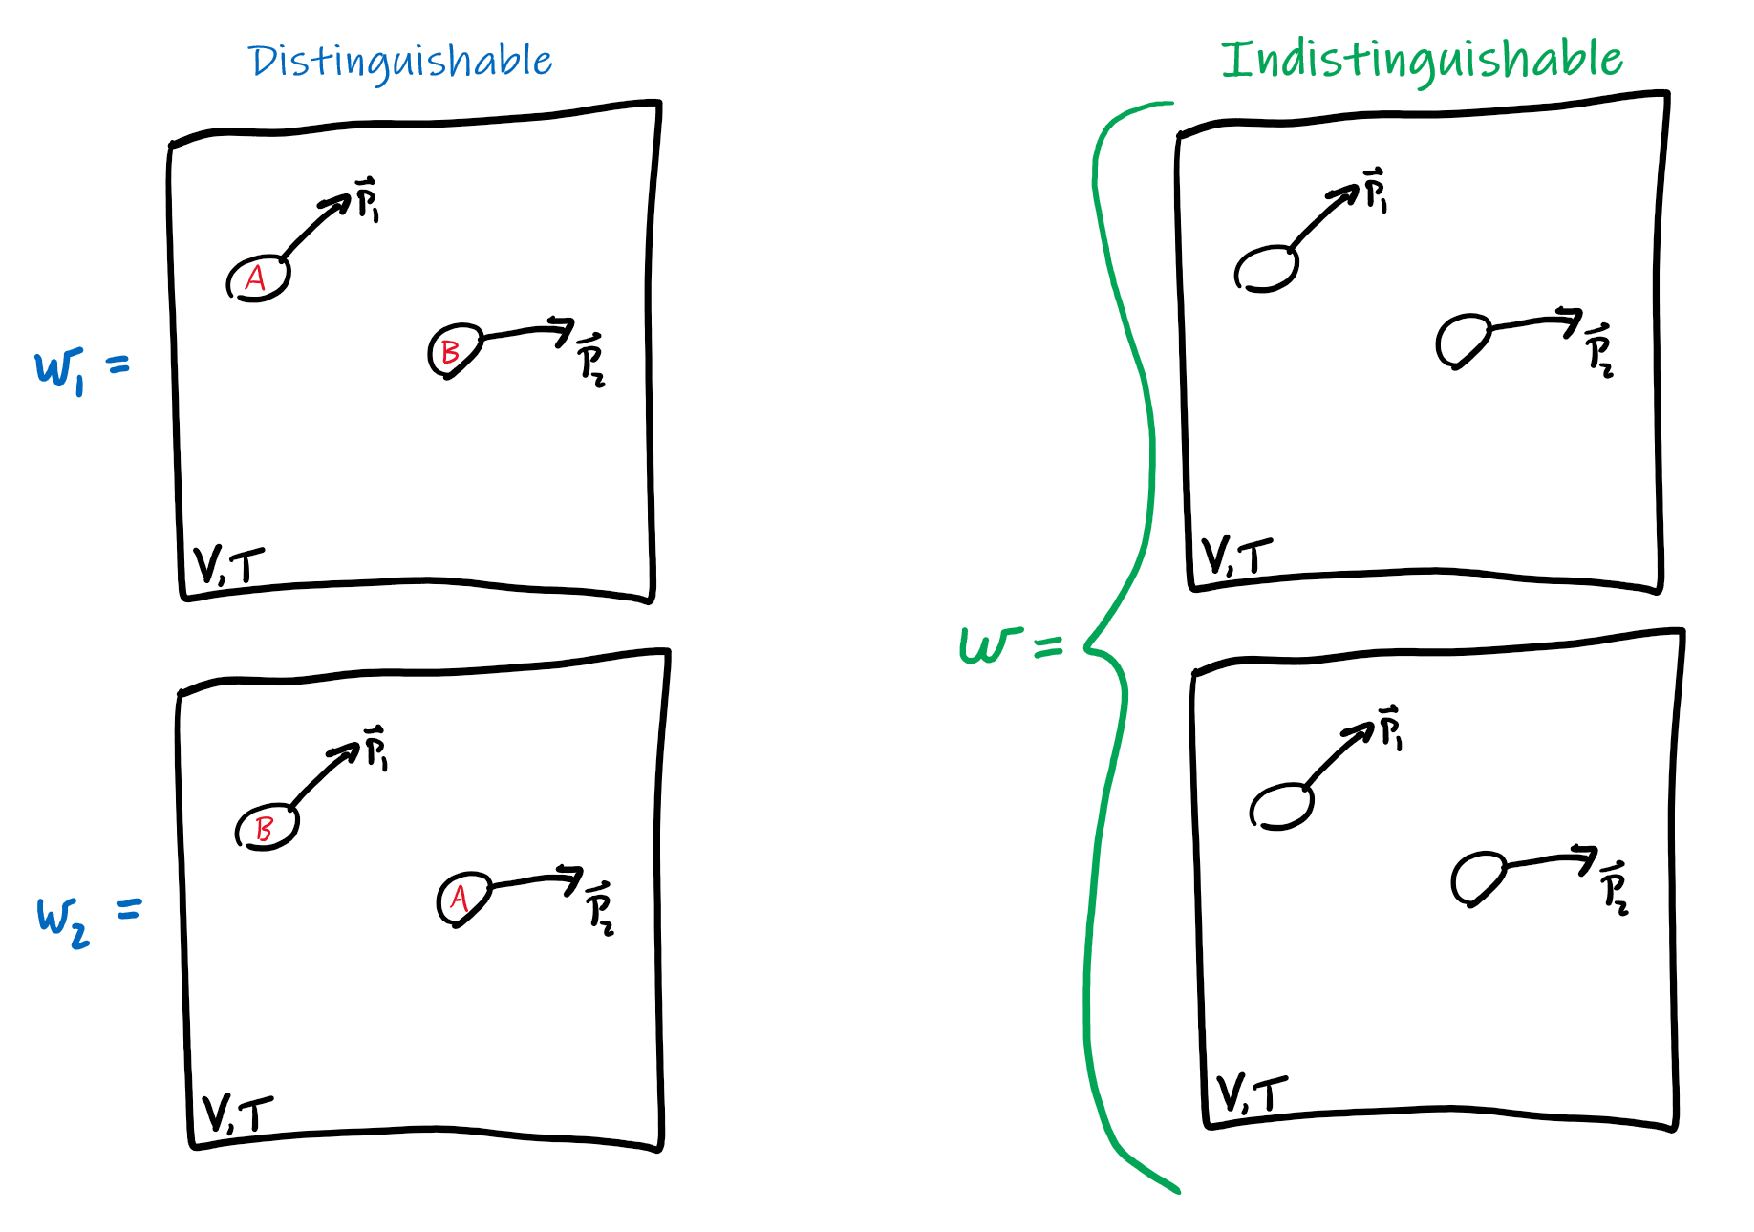
\includegraphics[width=0.7\textwidth]{figs/week04_distinguish.pdf}
\end{center}
If the particles are indistinguishable, no such labeling is possible, and there is only a single micro-state for these $\left\{\vec p_1, \vec p_2\right\}$, rather than two.
This factor of $2$ is not accidental, as you can check by counting how many micro-states there are for three distinguishable particles with momenta $\left\{\vec p_1, \vec p_2, \vec p_3\right\}$, compared to the single micro-state for the indistinguishable case:
\begin{mdframed}
  \ \\[100 pt]
\end{mdframed}

In full generality, ideal gases with distinguishable particles have
\begin{equation*}
  \binom{N}{1}\binom{N - 1}{1}\binom{N - 2}{1}\cdots\binom{1}{1} = N!
\end{equation*}
times more micro-states compared to otherwise-identical ideal gases with indistinguishable particles.
The partition function sums over these micro-states, but depends only on their energies, which are independent of any labeling.
Therefore this factor of $N!$ is the only difference between \eq{eq:ideal_dist} and the partition function $Z_I$ for indistinguishable particles,
\begin{equation}
  \label{eq:ideal_indis}
  Z_I = \frac{1}{N!} \left(\frac{mTL^2}{2\pi\hbar^2}\right)^{3N / 2} = \frac{1}{N!} \left(\frac{L}{\lath}\right)^{3N} = \frac{1}{N!} \left(\frac{V}{\lath^3}\right)^N.
\end{equation}
% ------------------------------------------------------------------



% ------------------------------------------------------------------
\subsection{Internal energy, and entropy}
Now that we have the partition function for a non-relativistic, classical, ideal gas in a box of volume $V = L^3$, let's apply our work from last week to find the average internal energy $\vev{E}$ and entropy $S$ for the gas.


\TODO{Being written...}
% ------------------------------------------------------------------



% ------------------------------------------------------------------
\newpage % TODO: Placeholder...
\subsection{The Gibbs paradox and the mixing entropy}
The `Gibbs paradox' was an argument presented by J.\ Willard Gibbs in 1874--1875 that seemed to show a way for the entropy of an isolated system to decrease, in violation of the second law of thermodynamics.
Here we will summarize the argument and point out where it goes wrong.

\TODO{Being written...}
% ------------------------------------------------------------------



% ------------------------------------------------------------------
\newpage % TODO: Placeholder...
\subsection{Pressure and the equation of state}
\TODO{Being written...}
% ------------------------------------------------------------------
